\chapter{Elixir}
Elixir is a dynamic, functional language for building scalable and maintainable applications \cite{elixir}. Elixir programs run on the BEAM virtual machine\cite{beam}, which is also used to implement the Erlang programming language \cite{erlang}. Elixir was designed by José Valim and first released in 2012. Elixir is built on top of Erlang and hence inherits many of the abstractions designed for building distributed systems.
\par
BEAM is a virtual machine that executes user programs in the Erlang Runtime System (ERTS). BEAM is a register machine where all instructions operate on named registers containing Erlang terms such as integers or tuples.
\par
Elixir has begun to see use in industry, in particular in domains such as telecoms and instant messaging. The Phoenix Framework \cite{phoenix} is a framework for building interactive web applications natively in Elixir that can take advantage of Elixir's multi-processing and fault tolerance to build scalable web applications. The audio and video communication application Discord \cite{discord} uses Elixir to manage its 11 million concurrent users and the Financial Times \cite{ft} have begun migrating from Java to Elixir to enjoy the much smaller memory usage by comparison.
\par
Elixir supports multi-processing in two key ways: nodes and processes. Each node is an instance of BEAM (a single operating system process), when an Elixir program is executed, a new instance of BEAM is instantiated for it to run on. In contrast, an Elixir process is not an operating system process. An Elixir process is lightweight in terms of memory and CPU usage (even in comparison to threads that many other programming languages favour). Elixir processes can run concurrently with one another and are completely isolated from one another. Elixir processes communicate via message passing.
\begin{lstlisting}[language=Elixir, xleftmargin=.2\linewidth, caption={An example of spawn/1 and spawn/4 in Elixir for spawning a new lightweight process and a new Elixir node}]
    # Spawn a new process
    spawn(fn -> 1 + 2 end)

    # Create a new BEAM instance
    Node.spawn(:"node1@localhost", MyModule, :start, [])
\end{lstlisting}
\section{Shared Memory and Message Passing}
Two key concepts in inter-process communication (IPC) are shared memory models and message-passing models. They are two techniques used to allow processes to send signals or share data between each other. In a shared memory model, a shared memory region is established in which multiple processes can read and write. Figure \ref{fig:shared_memory} shows a basic example of two processes that write to a shared in-memory array. Due to how often we see shared memory used in large-scale distributed systems, much work has been done in the verification of these systems using shared memory models. For example, Jon Mediero Iturrioz used Dafny \cite{dafny} to prove the correctness of concurrent programs that implement shared memory \cite{shared_memory_verification}. 
\begin{figure}[h]
    \centering
    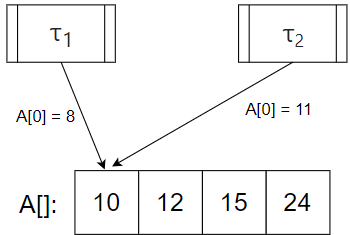
\includegraphics[width=0.4\textwidth]{images/shared_memory.png}
    \caption{An example of two processes writing to a shared in-memory array}
    \label{fig:shared_memory}
\end{figure}
\par
Elixir instead uses a message-passing model for IPC. More specifically, Elixir uses an actor-based model, where each process (actor) has its state and a message box to receive messages from other actors. Actors are responsible for sending a finite number of messages to other actors, spawning new actors and changing their behaviour based on the handling of messages received in the mailbox. Figure \ref{fig:actor_model} shows an example of how actors behave. The mailbox is not necessarily first in, first out (FIFO) but often implementations tend to be.
\begin{figure}[H]
    \centering
    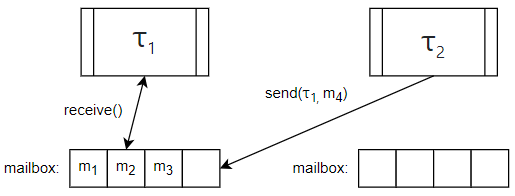
\includegraphics[width=0.6\textwidth]{images/actor_model.png}
    \caption{An example of actors sending and receiving messages under the actor model}
    \label{fig:actor_model}
\end{figure}
\par
In Elixir, a receive statement is used to read messages in the mailbox. The receive block looks through the mailbox for a message that matches a given pattern, if no messages match a given pattern, the process will block until one does.
\begin{lstlisting}[language=Elixir, xleftmargin=.4\linewidth, caption={An example of spawn/1 and spawn/4 in Elixir for spawning a new lightweight process and a new Elixir node}]
    # Example send in Elixir
    send self(), {:hello, "world"}

    # Example receive block in Elixir
    receive do
        {:hello, msg} -> IO.puts msg
    end
\end{lstlisting}
\section{Quote and Unquote}
The quote and unquote constructs in Elixir give us a deeper insight into how the programming language is implemented. Elixir is fundamentally made of tuples with three elements consisting of an atom\footnote{In Elixir, atoms are named constants, whose values are their own name. They can be identified by a preceding colon, for example, \texttt{:hello}.} that identifies the tuple, an array of metadata and finally the data. For example, the function call \texttt{sum(1, 2)} would be represented by the tuple \texttt{(:sum, [], [1, 2])} and similarly, the variable \texttt{total} would be represented by the tuple \texttt{(:total, [], Elixir)}. Using these building blocks, Elixir can begin to build what is known as a quoted expression, which is a nesting of tuples in a tree-like structure. In many other programming languages, this tree-like structure is referred to as an abstract syntax tree (AST).
\par
The quote and unquote constructs allow us to transition between Elixir syntax and quoted expressions. Using the \texttt{quote/2}\footnote{In Elixir, it is common to name functions or macros alongside their number of arguments. The function \texttt{spawn/1} refers to the function spawn, with 1 argument.} macro on an Elixir block, such as \texttt{quote do: sum(1, 2)} will return the quoted expression representing the block, in this case, \texttt{(:sum, [], [1, 2])}. Similarly, the \texttt{unquote/1} macro can be used within a quoted expression to inject code directly into the underlying expression. Figure \ref{fig:quote_unquote} shows a small example of how unquote can be applied within a quoted expression to inject a variable.
\begin{lstlisting}[language=Elixir, xleftmargin=.4\linewidth, caption={Elixir example of \texttt{quote/2} and \texttt{unquote/1}.}, label={fig:quote_unquote}]
    x = 2
    quote do: sum(1, unquote(x))
\end{lstlisting}
For ease of reading, we will use the terms quoted-expression and AST interchangeably for the remainder of the report.
\par

\section{Metaprogramming}
Metaprogramming is a technique that allows developers to write a program that outputs another program. It means a program can be designed to read or transform other programs. In Elixir, metaprogramming is often used to extend the language by directly modifying the generated quoted expressions by a program. This is achieved through the quote and unquote constructs alongside macros. Macros allow for transforming code and expanding a module.
\par
In Elixir, \texttt{defmacro/2} is used to define new macros, which itself is a macro. Macros receive quoted expressions as arguments and typically inject these expressions into code before returning another quoted expression. Listing \ref{fig:unless} introduces how \texttt{defmacro/2} can be used to define the \texttt{unless/2} macro used in the standard library. Unless is the opposite of an \texttt{if/2} statement, it will execute an expression if a conditional check evaluates to false.
\begin{lstlisting}[language=Elixir, xleftmargin=.3\linewidth, caption={Elixir example of the \texttt{unless/2} macro as defined in the standard library \cite{defmacro}}., label={fig:unless}]
defmacro unless(clause, do: expression) do
  quote do
    if(!unquote(clause), do: unquote(expression))
  end
end
\end{lstlisting}
\par
Macros are both lexical and explicit. That means it is impossible to inject macros globally and it is impossible to run macros without explicit invocation. By leveraging the use of functions, quoted expressions and macros, we can begin to develop a domain-specific language (DSL). For example, constructing a DSL that overrides the standard implementations for many Elixir constructs in a style that makes verifying the correctness of Elixir programs more trivial. By default, Elixir is very difficult to verify. Elixir provides an ExUnit module, with an \texttt{assert/1} macro which could be used for loop invariants, preconditions and postconditions but doesn't support an approach that favours writing verification-aware code. As many Elixir programs are concurrent, and as Elixir uses the actor model, verifying an arbitrary Elixir program that has not been restricted or extended using macros is a challenge.
\par
Another useful feature often associated with the development of DSLs in Elixir is attributes. Attributes can be used to store additional information, as a temporary storage. Attributes also work as constants, or simply to annotate code which can be useful for other developers or the virtual machine. Listing \ref{fig:attributes} shows a basic example of annotating a function with an attribute.
\begin{lstlisting}[language=Elixir, xleftmargin=.3\linewidth, caption={Example use of attributes in Elixir}., label={fig:attributes}]
    @doc "Calculate the sum of two numbers, x and y"
    def sum(x, y) do
        x + y
    end
\end{lstlisting}

\section{Additional Contructs}
Various other constructs in Elixir are useful to be aware of to understand the format of quoted expressions.
\subsection{Return Values and Types}
Elixir is a dynamically typed language, hence any introduced type specifications are never used by the compiler in optimisations or type-checks, however, using annotations\footnote{Annotations are used to add additional metadata to code. They are prefixed with an asperand, for example, \texttt{@type} or \texttt{@doc}.} Elixir does support type specification which can be relevant for documentation and additional tooling. Unlike many imperative programming languages where function return values must be explicitly defined using a keyword such as \texttt{return}, Elixir functions simply return the evaluation of a statement. This could also be the final statement if many statements are sequentially executed in a block.

\subsection{Charlists}
Elixir introduces linked lists as a data structure to store elements. Elixir lists are similar to other programming languages, where they are displayed as comma-separated values enclosed in square braces. If a list is made exclusively of non-negative integers, where every integer has a Unicode code point, then the list may be interpreted as a charlist. If the list contains only printable ASCII characters, then it is often stored and displayed in ASCII format. For example, the list \texttt{[97, 98, 99]} would be stored in the AST as \texttt{'abc'}.

\section{Summary}
In this chapter, we learned about Elixir, the programming language built on top of Erlang and we explored so basic approaches to designing concurrent systems with it. The next section will explore how these core tools can be used in tandem to provide developers guarantees over large-scale, distributed Elixir-based systems.